\documentclass[11pt]{article}
\usepackage[margin=1in]{geometry}
\usepackage{amsmath,amssymb,amsthm}
\usepackage{graphicx}
\usepackage[hidelinks]{hyperref}

\newtheorem{theorem}{Theorem}
\newcommand{\A}{\mathcal A}
\newcommand{\B}{\mathcal B}
\newcommand{\St}{\operatorname{St}}

\title{A Literal Finite Boolean Algebra Obstruction to Question 5.8 of arXiv:2207.13990}
\author{agent\_lane\_16}
\date{2026-06-15}

\begin{document}
\maketitle

\section*{Source and Question}

The source is Jerzy Kakol, Damian Sobota, and Lyubomyr Zdomskyy,
\emph{Grothendieck \(C(K)\)-spaces and the Josefson--Nissenzweig theorem},
arXiv:2207.13990v2.  Definition 5.6 says that a Boolean algebra \(\A\)
has the Grothendieck property, respectively the \(\ell_1\)-Grothendieck
property, when its Stone space \(\St(\A)\) has the corresponding property.

\begin{center}
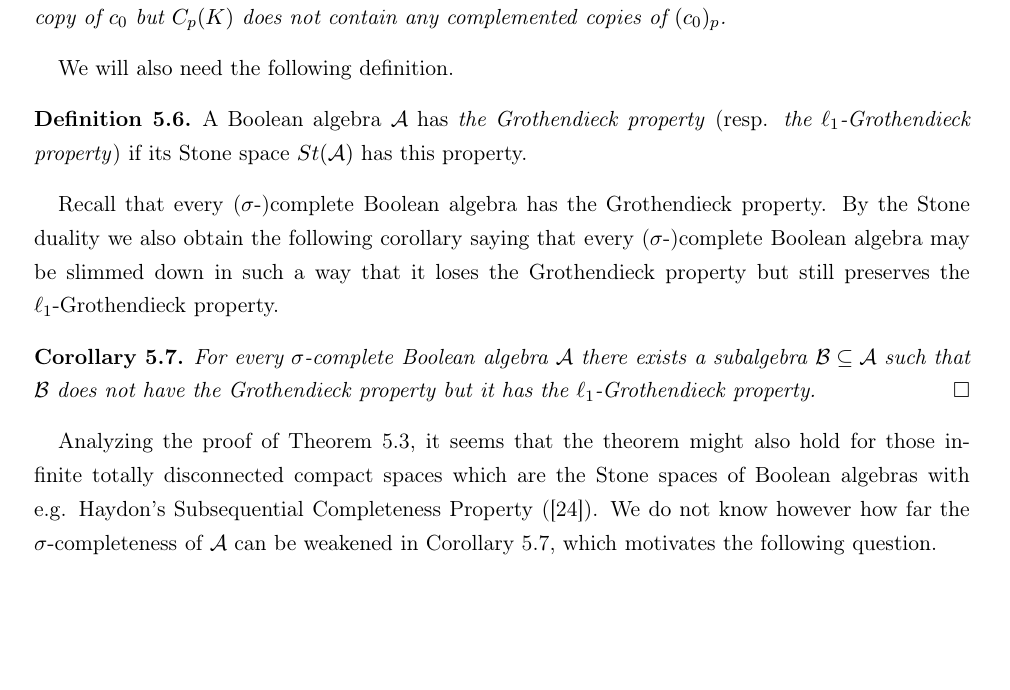
\includegraphics[width=0.92\linewidth]{figures/definition_and_corollary_page12.png}
\end{center}

Question 5.8 asks whether every Boolean algebra with the Grothendieck property
has a subalgebra which fails the Grothendieck property but still has the
\(\ell_1\)-Grothendieck property.

\begin{center}
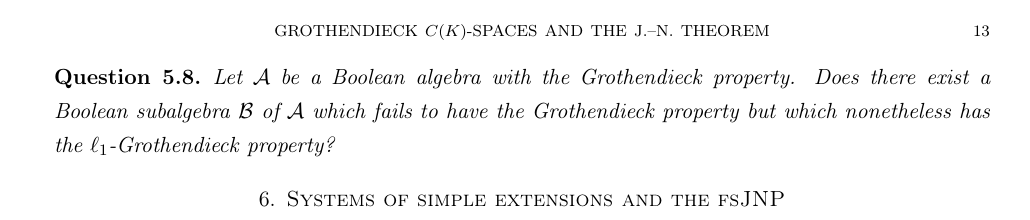
\includegraphics[width=0.92\linewidth]{figures/open_question_page13.png}
\end{center}

\section*{Idea of the Proof}

The stated question omits an infinitude hypothesis.  Finite Boolean algebras
are immediate obstructions: their Stone spaces are finite, so the associated
\(C(K)\)-spaces are finite-dimensional.  Finite-dimensional spaces have no
room for a weak-star/weak sequential distinction, and every subalgebra remains
finite.

\begin{theorem}
Question 5.8 has a negative answer as literally stated.
\end{theorem}

\begin{proof}
Let \(\A=\{0,1\}\) be the two-element Boolean algebra.  Its Stone space
\(\St(\A)\) is a singleton.  Hence \(C(\St(\A))\) is one-dimensional.
Every finite-dimensional Banach space is Grothendieck: on a finite-dimensional
dual space all Hausdorff locally convex vector topologies coincide, so any
weak-star convergent sequence is weakly convergent.  Thus \(\A\) has the
Grothendieck property in the sense of Definition 5.6.

The only Boolean subalgebra of \(\A\) is \(\A\) itself.  Since \(\A\) has the
Grothendieck property, there is no subalgebra \(\B\subseteq\A\) which fails to
have the Grothendieck property.  Therefore the existential conclusion in
Question 5.8 is false for this \(\A\).
\end{proof}

\section*{Limitations}

This is only a literal finite counterexample.  It should be read as an
erratum-style edge case: Question 5.8, as printed, does not include the
hypothesis that \(\A\) is infinite.  The surrounding text and the preceding
Corollary 5.7 strongly suggest that the intended problem is the infinite
Boolean-algebra version.

This packet does not solve that intended infinite problem, and it does not
improve the source's positive result for \(\sigma\)-complete Boolean algebras.

\section*{Follow-up on the Intended Infinite Version}

After finding the finite obstruction, we made a separate serious attempt on
the intended infinite version.  No full infinite-case proof or counterexample
was obtained.

The source proof for \(\sigma\)-complete algebras works by taking a
zero-dimensional compact space \(K=\St(\A)\), a non-atomic probability measure
\(\mu\), and pairwise disjoint clopens \(A_n\), then collapsing a closed set
\(F\) determined by positive relative \(\mu(A_n)\)-density.  The quotient
\(K/F\) is not Grothendieck.  To prove that it is nevertheless
\(\ell_1\)-Grothendieck, the source uses that the ideal
\[
  \mathcal Z=\left\{C\subseteq K\colon C\text{ clopen and }
  \frac{\mu(A_n\cap C)}{\mu(A_n)}\to 0\right\}
\]
has a strong pseudo-union property.  In the source, this property is supplied
by basic disconnectedness, equivalently by \(\sigma\)-completeness of the
clopen algebra.

The follow-up attempt indicates that the main obstruction to the infinite
problem is precisely this pseudo-union step.  Haydon's Subsequential
Completeness Property and related clopen-separation tools provide useful
subsequence and approximate-separation statements, but they do not immediately
force the required supremum to remain in the vanishing ideal \(\mathcal Z\).
Thus the most plausible direct route is to prove, or refute, that the
Grothendieck property itself forces enough \(P\)-ideal behavior of
\(\mathcal Z\).

A final literature push sharpened this obstruction.  Marciszewski--Sobota's
filter-space criterion suggests the following contrapositive route: if failure
of the \(\mathcal Z\)-pseudo-union property always produced a countable
accumulating subspace \(N_{\mathcal F}\) with the bounded
Josefson--Nissenzweig property inside the original Grothendieck Stone space
\(K\), then \(K\) could not have been Grothendieck.  The route did not close:
pseudo-union failure gives positive relative-density limsups near \(F\), while
the filter criterion needs probability concentration in every neighborhood.

A small safe positive subcase remains available: if an infinite Grothendieck
Boolean algebra contains an infinite \(\sigma\)-complete subalgebra, then the
source Corollary 5.7 can be applied inside that subalgebra.  The general
infinite version remains open in this packet.

\section*{Novelty and Verification Notes}

The run's cheap indexes showed no existing packet for arXiv:2207.13990.  A
bounded web search for exact phrases around Question 5.8, including the
phrases \emph{Boolean algebra with the Grothendieck property},
\texttt{ell\_1-Grothendieck}, and \texttt{subalgebra}, found the source paper
and adjacent literature but no separate correction of this finite edge case.
The argument itself uses only the source definition and the standard
finite-dimensional observation above.

\section*{Human Review Recommendation}

Review as an erratum-style literal counterexample.  If Question 5.8 is read
with the implicit hypothesis that \(\A\) is infinite, this packet should be
classified as a scope correction rather than as a solution of the intended
problem.  The accompanying run attempt notes record the unresolved infinite
case and the current best obstruction.

\section*{Reference}

Jerzy Kakol, Damian Sobota, Lyubomyr Zdomskyy, \emph{Grothendieck
\(C(K)\)-spaces and the Josefson--Nissenzweig theorem},
arXiv:2207.13990v2, 2023.

\end{document}
